% Copyright (c) 2022 by Lars Spreng
% This work is licensed under the Creative Commons Attribution 4.0 International License. 
% To view a copy of this license, visit http://creativecommons.org/licenses/by/4.0/ or send a letter to Creative Commons, PO Box 1866, Mountain View, CA 94042, USA.

%~~~~~~~~~~~~~~~~~~~~~~~~~~~~~~~~~~~~~~~~~~~~~~~~~~~~~~~~~~~~~~~~~~~~~~~~~~~~~~
% You can add your packages and commands to the loadslides.tex file. 
% The files in the folder "styles" can be modified to change the layout and design of your slides.
% I have included examples on how to use the template below. 
% Some of these examples are taken from the Metropolis template.
%~~~~~~~~~~~~~~~~~~~~~~~~~~~~~~~~~~~~~~~~~~~~~~~~~~~~~~~~~~~~~~~~~~~~~~~~~~~~~~


\documentclass[
11pt,notheorems,hyperref={pdfauthor=whatever}
]{beamer}

\input{loadslides.tex} % Loads packages and some defined commands

\title[
Chemistry of Forest Fires and Regional Haze
]{Chemistry of Forest Fires and Regional Haze \\ With emphasis on Southeast Asia }
\subtitle{Based on \citet{radojevic2003chemistry}}


\author[
% Text entered here will appear in the bottom left corner
]{
    Nathasya Christien 
}

\institute{
    Biogeochemical Cycles Course \\
    Earth System Physics \\
    ICTP}
\date{June 16, 2026}

\begin{document}

% Generate title page
{
\setbeamertemplate{footline}{} 
\begin{frame}
  \titlepage
\end{frame}
}
\addtocounter{framenumber}{-1}

% \begin{frame}{Outline}
%     \tableofcontents
% \end{frame}

\section{Introduction}
\begin{frame}
    \begin{itemize}
        \begin{columns}[T,onlytextwidth]
        \column{0.5\textwidth}
            \centering
            {
            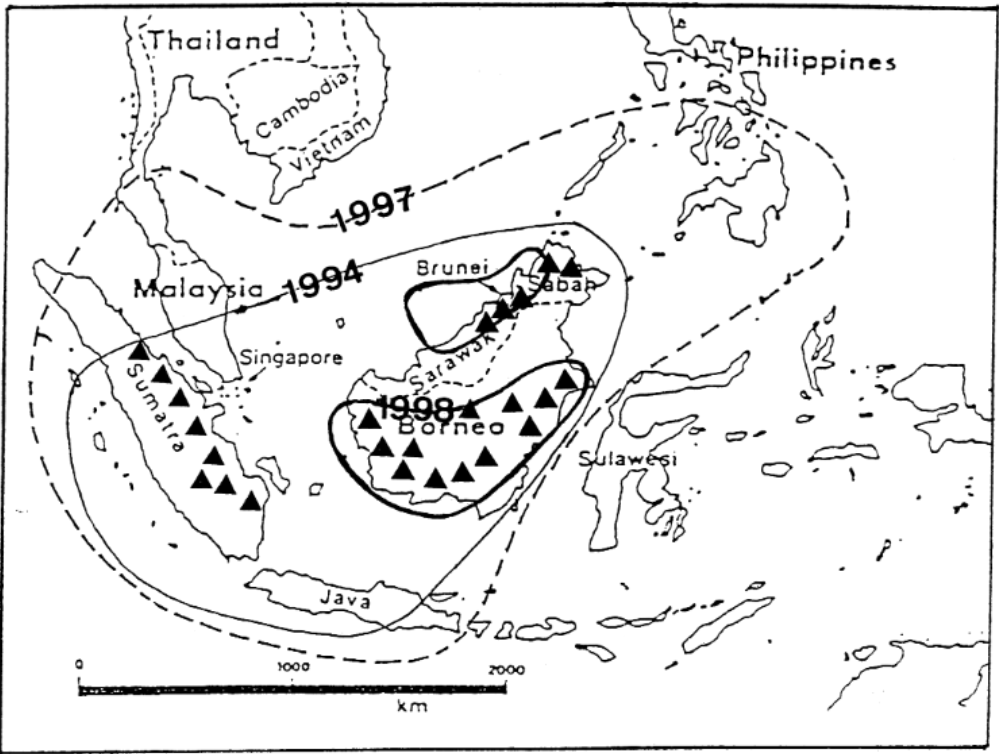
\includegraphics[width=1.0\textwidth]{figs/se_asia.png}
            \vspace{0.2cm}
            {
                \scriptsize 
                Location of forest fire hot-spots ($\blacktriangle$) and extent of regional haze
            }
            }
        
        \column{0.45\textwidth}
        \item Forest fires in the tropics consume up to 80\% of the total biomass burned on a global scale.
        \item Haze: a regional air pollution phenomenon caused by biomass fires' emission.
        \item Impacts include health, biogeochemical cycles, weather and climate, tropospheric ozone, and rainwater acidity.
        \item Forest firest in SE Asia affect one of the most densely populated regions of the world.
        \item Drivers: Often triggered by El Niño-induced droughts and deliberate land-clearing "slash and burn" practices
        \end{columns}
    \end{itemize}
\end{frame}

\section{Biomass Combustion Chemistry}
\begin{frame}
    \begin{itemize}
        \item Fuel: vegetation, peat and lignite coal.
    \end{itemize}

    % \begin{block}{Stages of forest fire}
    %     \centering
    %     Ignition $\rightarrow$ Flaming $\rightarrow$ Smouldering $\rightarrow$ Extinction
    % \end{block}

    \begin{block}{Flaming Stage}
        \begin{itemize}
            \item Characterised by \textbf{high temperatures} (\qty{1800}{\kelvin}) and \textbf{visible} flames, under high oxgen concentrations.
            \item Emissions rich in \ce{H2O}, \ce{CO2}, \ce{NO}, \ce{N2O}, and \ce{N2}, along with particles high in elemental carbon. Reactions tend to completion and oxidised forms are released.
        \end{itemize}
    \end{block}

    \begin{block}{Smouldering Stage}
        \begin{itemize}
            \item Characterised by \textbf{lower temperatures} and \textbf{without any visible} flames
            \item Emits incompletely oxidised compounds: \ce{CO}, \ce{CH4}, non-methane hydrocarbons, PAHs, and VOCs.
        \end{itemize}
    \end{block}

    \begin{block}{Main emissions}
        \begin{itemize}
            \item More than 95\% of carbon emitted by biomass fires is in form of \ce{CO} and \ce{CO2}.
            \item Emitted smoke particles are generally less than \qty{10}{\micro\metre} in diameter.
        \end{itemize}        
    \end{block}
\end{frame}

\section{Biomass Combustion Studies}

\begin{frame}
    \begin{itemize}
        \item Methodology: 
        \begin{itemize}
            \item laboratory studies
            \item field measurements
            \item numerical modelling (\underline{satellite observations} as input of \underline{dispersion model}, which then be verified using \underline{ground-based observations})
        \end{itemize}
        
    \end{itemize}

    \begin{block}{Field Study in SE Asia (Brunei)}
        \begin{itemize}
            \item Criteria Pollutants: Standard monitoring focus is on \ce{PM_{10}}, \ce{SO2}, \ce{NO2}, \ce{CO}, and \ce{O3}.
            \item Aerosol Size: Particle size analysis shows that >99\% of haze particles are \ce{PM_{2.5}}, making them "respirable" and highly hazardous to health.
            \item Suspended particle concentrations, leading to visible impacts: 
            
            \begin{itemize}
                \item \ce{C} was the major constituent, present at 50--70\% of the aerosol mass.
                \item K is identified as a primary tracer for biomass burning, making up 10–20\% of the aerosol mass in SE Asian haze
            \end{itemize}
        \end{itemize}
    \end{block}
\end{frame}

\section{Tropospheric Chemistry and Secondary Ozone Formation}

\begin{frame}
    % \begin{itemize}
    %     \item As haze travels, primary pollutants are converted into secondary pollutants via chemical reactions.
    %     \item Tropospheric chemistry is more active given greater solar intensity and higher temperatures in the tropics.
    % \end{itemize}

    \begin{block}{Radical Generation}
        \[ \ce{O3 + h$\nu$ ($\lambda < \qty{315}{\nano\meter}$) -> O2 + O(^1D)} \]
        \[\ce{ O(^1D) + H2O -> 2OH${}^\cdot$ }\]
    \end{block}

    \begin{block}{Ozone Production}
        \[ \ce{NO2 + h$\nu$ -> NO + O(^3P)} \]
        \[ \ce{O(^3P) + O2 + M -> O3 + M} \]
    while 
        \[ \ce{NO + O3 -> NO2 + O2} \]
    \end{block}

    \begin{block}{The Haze Paradox}
        Under steady state,
        $$
        [\ce{O3}] = J \,[\ce{NO2}] / k \,[\ce{NO}]
        $$
        In thick haze, the photodissociation constant (J) is reduced because smoke blocks solar radiation, effectively "shutting down" \ce{O3} production.
    \end{block}
\end{frame}

\section{Impacts on Rainwater Chemistry}

\begin{frame}
    \begin{block}{Findings in SE Asia}
        \begin{itemize}
            \item Brunei Darussalam (Haze episodes of 1994, 1997, 1998): Comparison of the pH of individual rainwater samples revealed \textbf{no significant acidification}.
            \item Singapore (Haze episode of 1997): Similar conclusion.
        \end{itemize}
    \end{block}

    \begin{block}{Neutralization Mechanism}
        Acidifying compounds (e.g \ce{SO2}, \ce{NO_x}) are neutralized by alkaline substances (\ce{Ca}, \ce{Mg}, \ce{K}) leached from smoke particles into cloud water.
    \end{block}

    \begin{block}{Deposition Rates}
        \begin{itemize}
            \item While haze increases the ionic content of individual rain samples, total annual acid deposition remains low because the fires occur during the dry season when precipitation is minimal.
            \item The monthly contributions during periods of forest fires and haze to \ce{H^+} in Brunei is small, indicating a minor source of acidity in wet deposition.
        \end{itemize}
    \end{block}
\end{frame}

\section{Impacts on Weather and Climate}

\begin{frame}
    \begin{block}{Greenhouse Gases}
        \begin{itemize}
            \item Biomass burning is a significant global source of \ce{CO2} and \ce{CH4}.
            \item Larger contributor to global carbon emissions after fossil fuel combustion in industrialised countries.
        \end{itemize}
    \end{block}

    \begin{block}{Affecting The Earth's Radiation Balance}
        \begin{itemize}
            \item Less solar heating at the Earth's surface due to scattering and absorption from smoke particles.
            \item Reduced ambient temperatures were observed in Sarawak, Malaysia following 1997 episode.
            % \item Photosynthetically active radiation (PAR) was severely reduced, while relative humidity was higher on haze days compared to clear days.
        \end{itemize}
    \end{block}

    \begin{block}{Cloud Condensation Nuclei (CCN)}
        Non-activated particles may compete for available water vapor, increasing cloud stability and decreasing precipitation.
    \end{block}

    \medskip
    \centering
    \textit{"At present (2003), the probable effects ... are at best speculative."}
\end{frame}

\section{Concluding Remarks}
\begin{frame}
    \begin{itemize}
        \item SE Asian haze is dominated by PM${}_{2.5}$, inhibited photochemistry, neutralized rainwater acidity.
        \item These theories help us facing the coming El Niño event, which usually drives the forest fire.
    \end{itemize}
\end{frame}


% \begin{frame}[allowframebreaks]{References}
%     \printbibliography
% \end{frame}
\end{document}